\begin{XeClass}{FileStatus}
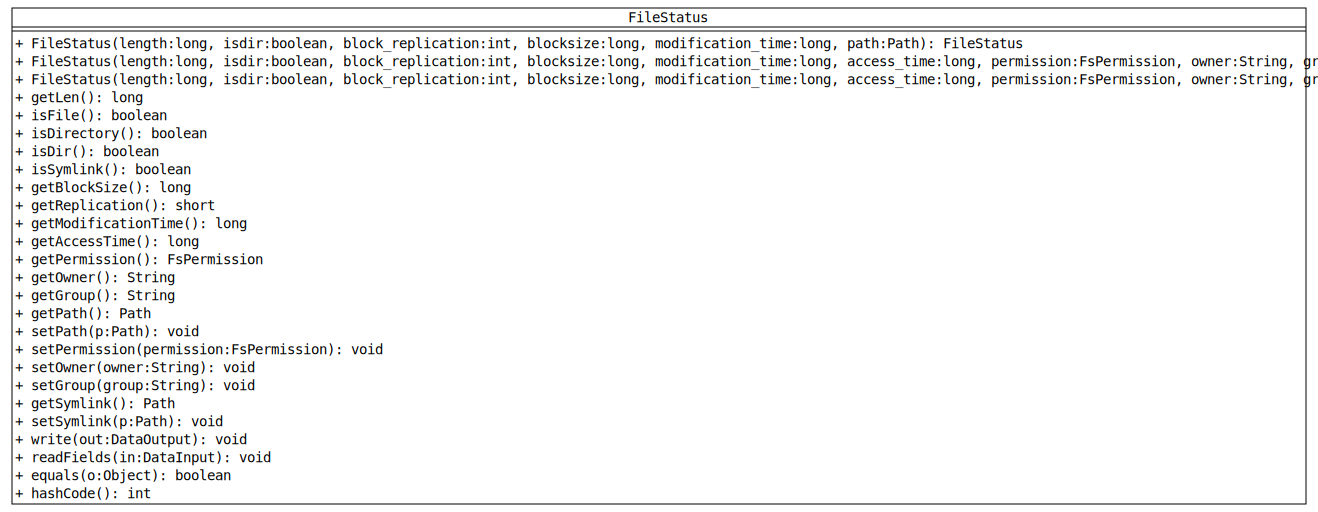
\includegraphics[width=\textwidth]{cdig/FileStatus.png}
     
 该类抽象提供了文件信息的抽象,屏蔽了具体文件系统的具体实现。
 文件的状态信息具体包含有文件路径、文件长度、是否是目录、复制块大小、
 块大小、修改时间、访问时间、权限、拥有者、所属的组、符号链接等

    \begin{XeMethod}{\XePublic}{FileStatus}{FileStatus}
         
 构造函数的另一个版本,包装了主要的构造函数来实现,即将被抛弃

    \end{XeMethod}

    \begin{XeMethod}{\XePublic}{FileStatus}{FileStatus}
         
 构造函数的另一个版本,包装了主要的构造函数来实现

    \end{XeMethod}

    \begin{XeMethod}{\XePublic}{FileStatus}{FileStatus}
         
 构造函数,设置了此文件的基本参数

    \end{XeMethod}

    \begin{XeMethod}{\XePublic}{long}{getLen}
         
 返回文件的字节长度

    \end{XeMethod}

    \begin{XeMethod}{\XePublic}{boolean}{isFile}
         
 判断此文件是否为文件,以区别文件目录和文件链接

    \end{XeMethod}

    \begin{XeMethod}{\XePublic}{boolean}{isDirectory}
         
 判断是否为文件目录

    \end{XeMethod}

    \begin{XeMethod}{\XePublic}{boolean}{isDir}
         
 判断是否为文件目录,此方法将被isDirectory代替。

    \end{XeMethod}

    \begin{XeMethod}{\XePublic}{boolean}{isSymlink}
         
 判断是否为文件链接

    \end{XeMethod}

    \begin{XeMethod}{\XePublic}{long}{getBlockSize}
         
 返回文件的块大小

    \end{XeMethod}

    \begin{XeMethod}{\XePublic}{short}{getReplication}
         
 返回文件的副本数量

    \end{XeMethod}

    \begin{XeMethod}{\XePublic}{long}{getModificationTime}
         
 返回文件的修改日期

    \end{XeMethod}

    \begin{XeMethod}{\XePublic}{long}{getAccessTime}
         
 返回文件的创建时间

    \end{XeMethod}

    \begin{XeMethod}{\XePublic}{FsPermission}{getPermission}
         
 取得文件的权限,如果文件系统不支持权限,则返回 777(rwxrwxrwx)

    \end{XeMethod}

    \begin{XeMethod}{\XePublic}{String}{getOwner}
         
 返回文件的所有者,如果文件系统不支持所有者,则返回null

    \end{XeMethod}

    \begin{XeMethod}{\XePublic}{String}{getGroup}
         
 返回文件所在的工作组,如果文件系统不支持工作组,则是未定义行为

    \end{XeMethod}

    \begin{XeMethod}{\XePublic}{Path}{getPath}
         
 返回文件的路径

    \end{XeMethod}

    \begin{XeMethod}{\XePublic}{void}{setPath}
         
 设置文件的路径

    \end{XeMethod}

    \begin{XeMethod}{\XeProtected}{void}{setPermission}
         
 设置文件权限

    \end{XeMethod}

    \begin{XeMethod}{\XeProtected}{void}{setOwner}
         
 设置文件所有者,默认为""

    \end{XeMethod}

    \begin{XeMethod}{\XeProtected}{void}{setGroup}
         
 设置文件所在工作组,默认为""

    \end{XeMethod}

    \begin{XeMethod}{\XePublic}{Path}{getSymlink}
         
 如果此文件是链接,则获取该链接

    \end{XeMethod}

    \begin{XeMethod}{\XePublic}{void}{setSymlink}
         
 设置文件链接

    \end{XeMethod}

    \begin{XeMethod}{\XePublic}{void}{write}
         
 向指定的流输出文件的基本信息

    \end{XeMethod}

    \begin{XeMethod}{\XePublic}{void}{readFields}
         
 从给定的流读取并设置该文件的属性

    \end{XeMethod}

    \begin{XeMethod}{\XePublic}{boolean}{equals}
         
 通过判断路径是否相等来判断此文件和给定的文件是否相同

    \end{XeMethod}

    \begin{XeMethod}{\XePublic}{int}{hashCode}
         
 返回此文件的hash码,即文件的路径的hash码

    \end{XeMethod}

\end{XeClass}
